\chapter{Metastable phase study in the Ti-Ta and Ti-Nb systems}

\section{Introduction}

The present chapter is aimed at studying the formation of the metastable phases $\omega$ and $\alpha"$. As shown in Figures \ref{Ch1-figure:titaelastic} and \ref{Ch1-figure:tinbelasitc}, the formation of the $\alpha"$ and $\omega$ phases affects the elastic properties of Ti-Ta and Ti-Nb alloys. Currently the CALPHAD method predicts the equilibrium phase formation. For Ti-Nb, the CALPHAD method predicts that the alloys will form either the single hcp or bcc phases or a two-phase mixture of bcc and hcp. Understanding the effect of the metastable phases on the elastic properties and being able to predict at what compositions they form, will help with alloy selection and increase the likelihood of finding a suitable alloy for load-bearing implants. The stability of the bcc, hcp, $\omega$, and $\alpha"$ phases at 0 $^\circ$K is calculated and discussed for the Ti-Ta and Ti-Nb alloys using multiple structures across the entire composition range. The elastic properties of the four phases are then calculated systematically and interaction parameters are introduced using the CALPHAD method, similar as described in chapter 5, to be able to predict the elastic properties as a function of composition. With an understanding of how the phases affect the elastic properties, an adaptation of the partition function approach, was introduced (in chapter 2) to be able to predict the formation of the metastable phases. In order to ensure the accuracy of the theoretic framework, neutron scattering experiments are completed on 4 different Ti-Nb compositions. The data from the experiments is used to determine the phase fractions and phonon density of states. The results from the neutron scattering are compared with the theoretical results. The determined phase fractions are used to predict the elastic properties and compared with experimental values in the literature.

\section{Modeling and Calculations}

\subsection{Computational details}

In the present work, the Vienna ab-initio Simulation Package (VASP) \cite{Kresse1996} was employed to calculate the ground state energy and elastic properties of the pure elements and Ti-Nb and Ti-Ta systems in the bcc, hcp, $\omega$, and $\alpha"$ phases. The ion-electron interactions were described using the projector augmented wave (PAW) \cite{Kresse1999,Blochl1994} method and based on the previous work of comparing X-C functionals (Figure \ref{Ch5-figure:PBEvsPW91}) the exchange-correlation functional of the generalized gradient approach depicted by Perdew, Burke, and Ernzerhof (PBE-GGA) was employed \cite{Perdew1996a}. The energy convergence criterion of the electronic self-consistency was set as 10$^{-6}$ eV/atom. Indepedent structures based on the ATAT code were generated for the four phases, bcc (330), hcp (21), $\alpha"$ (33) and $\omega$ (73), across the entire composition range, were calculated. The Brillouin zone sampling was done using the $\Gamma$-centered Monkhorst-Pack scheme \cite{Monkhorst1976a}. The k-points grid for the hcp, $\omega$ and $\alpha"$ phases were 10x10x13, 13x13x7, and 12x11x10, respectively. The k-point grids fro the bcc calculations used the automated k-point mesh generator in VASP with the length of the subdivisions specificed as 50. The elastic properties were then calculated using a $\pm$0.01 magnitude of strain.

\subsection{Modeling details}

The elastic stiffness constants were modeled using the first-principles based DFT results. The modeling was completed by the methodology outlined in chapter 2. The difference between the first-principles calculations and the linear combination from the pure elements was caculated and the fittings were completed and the interaction parameters were fit using the code in appendix C. The best fit was found by comparing the fittings obtained with one interaction parameter or with two interaction parameters. The moduli values were than calculated using pycalphad and the code in appendix D and E \cite{Otis2017}.

\section{Results and discussion}

\subsection{First-principles calculations at 0 $^\circ$K}

The phase stability at 0 $^\circ$K is calculated as a function of composition for the Ti-Nb and Ti-Ta systems. Figure \ref{Ch7-figure:tinb0K} and \ref{Ch7-figure:titab0K} show the relative energy of the bcc, hcp, $\omega$, and $\alpha"$ phases from 100 at. \% Ti to 100 at. \% Nb or Ta. The relative energies are calculated according to Eq. \ref{eq: hform} using the ground state energies of the pure elements in the SER state as reference. Figure \ref{Ch7-figure:titab0K} is the relative energy of the bcc, hcp, $\omega$, and $\alpha"$ phases from 100 at. \% Ti to 100 at. \% Ta. Figure \ref{Ch7-figure:tinb0K} and \ref{Ch7-figure:titab0K} are both at 0 $^\circ$K. The calculations are still ongoing for Figure \ref{Ch7-figure:tinb0K}. The figures show that the relative energy of the hcp phase starts negative and then increases to pure Nb or Ta. The bcc phase starts with a higher relative energy at pure Ti and then decreases to negative at pure Nb or Ta. The hcp phase is lower relative energy to 30 at. \% Nb when the bcc phase has a lower relative energy. The $\omega$ and $\alpha"$ have similar relative energies at pure Ti and some of the structures continue to have similar relative energies from pure Ti to 80 at. \% Nb or Ta. The phases may be metastable and stabilized with by entropy.

Kim et al.  \cite{Kim2006} figured out the martensitic transformation temperature for Ti-Nb alloys between 20 and 30 at. \% Nb, shown in Figure \ref{Ch7-figure:titnbms}. Based on this available information, the Ti-Nb system is studied more in depth in the remaining parts of this chapter. 

\subsection{Elastic properties}

For the Ti-Nb system, the elastic stiffness constants of the bcc, hcp, $\alpha"$, and $\omega$ phases are calculated. The calculations and interaction parameters of the bcc phase are discussed in chapter 5. Figure \ref{Ch7-figure:adpelas1} and \ref{Ch7-figure:adpelas2} plot the elastic stiffness constants, $c_{11}$, $c_{12}$, $c_{13}$, $c_{22}$, $c_{23}$, $c_{33}$, $c_{44}$, $c_{55}$, and $c_{66}$, for the $\alpha"$ phase. The plots show the first-principles results (circles), the linear combination from the pure elements (dashed red line) and the fitting (solid line) using the interaction parameters in Table \ref{Ch7-table:intpara}. The $c_{11}$ and $c_{22}$ values decrease at first to 25 at. \% Nb then increase to 95 at. \% Nb and finally decrease (in value) from 95 at. \% Nb to pure Nb. The $c_{12}$ values increase to 40 at. \% Nb and then decrease from 40 at. \% Nb to pure Nb. The $c_{13}$ values increase to 30 at. \% Nb, then decrease to 80 at. \% Nb and then increase (in value) from 80 at. \% Nb to pure Nb. The $c_{23}$ values decrease at first to 25 at. \% Nb and then increase from 25 at. \% Nb to pure Nb. The $c_{33}$ values decrease from pure Ti to 50 at. \% Nb and then increase from 50 at. \% Nb to pure Nb. The $c_{44}$ values increase from pure Ti to pure Nb. The $c_{55}$ values decrease from pure Ti to 20 at. \% Nb, then increase to 65 at. \% Nb and then decrease from 65 at. \% Nb to pure Nb. The $c_{66}$ decreases in value from pure Ti to 60 at. \% Nb then increases to 85 at. \% Nb and then decrease to pure Nb.

Figure \ref{Ch7-figure:omegae1} plots the elastic stiffness constants, $c_{11}$, $c_{12}$, $c_{13}$, $c_{33}$, and $c_{44}$, for the $\omega$ phase. The plots show the first-principles results (circles), the linear combination from the pure elements (dashed red line) and the fitting (solid line) using the interaction parameters in Table \ref{Ch7-table:intpara}. The $c_{11}$ values decrease from pure Ti to 25 at. \% Nb and then increase to pure Nb. The $c_{12}$ values increase from pure Ti to 10 at. \% Nb, then decrease to 65 at. \% Nb and then increase from 65 at. \% Nb to pure Nb. The $c_{13}$ values increase from pure Ti to 70 at. \% Nb and then decrease to pure Nb. The $c_{33}$ values decrease from pure Ti to 25 at. \% Nb, then increase to 80 at. \% Nb and then decrease to pure Nb. The $c_{44}$ values decrease from pure Ti to 20 at. \% Nb, then increase (in value) from 20 to 70 at. \% Nb and then decrease from 70 at. \% Nb to pure Nb.

Figure \ref{Ch7-figure:hcpe1} plots the elastic stiffness constants, $c_{11}$, $c_{12}$, $c_{13}$, $c_{33}$, and $c_{44}$, for the hcp phase. The plots show the first-principles results (circles), the linear combination from the pure elements (dashed red line) and the fitting (solid line) using the interaction parameters in Table \ref{Ch7-table:intpara}.The $c_{11}$ values increase from pure Ti to 10 at. \% Nb and then decreases from 10 to 70 at. \% Nb and then increases from 70 at. \% Nb to pure Nb. The $c_{12}$ values decrease from pure Ti to 10 at. \% Nb and then increase from 10 at. \% Nb to pure Nb. The $c_{13}$ values decrease from pure Ti to 10 at. \% Nb, then increase from 10 to 75 at. \% Nb and then decrease (in value) from 75 at. \% Nb to pure Nb. The $c_{33}$ values decrease from pure Ti to 45 at. \% Nb, then increase from 45 at. \% Nb to pure Nb. The $c_{44}$ values decrease from pure Ti to 10 at.\% Nb, then increase to 75 at. \% Nb and then decrease from 75 at. \% Nb to pure Nb.

The interaction parameters determined are listed in \ref{Ch7-table:intpara} and the calculated elastic stiffness constants and $E$ values are listed in Table \ref{Ch7-table:tinbdata}. The Young's moduli values are calculated as a function of composition and are plotted in Figure \ref{Ch7-figure:tinbelastic}. The dotted lines are the fittings that use the interaction parameters in Table \ref{Ch7-table:intpara}. The calculations show that the Young's moduli for the hcp phase decrease (in value) from pure Ti (124 GPa) until 60 at. \% Nb (-78 GPa) and then increase from 80 at. \% Nb to pure Nb (15 GPa). The Young's moduli, for the $\omega$ phase, follows the same trend as the hcp phase. The $E$ values decrease from pure Ti (152 GPa) to around pure Nb (-158 GPa). The $E$ values for the bcc phase increase from -40 GPa at pure Ti to 98 GPa at pure Nb. The $E$ values for the $\alpha"$ phase decrease from 133 GPa at pure Ti to 94 GPa at 20 at. \% Nb, then increase to 138 GPa 70 at. \% Nb and then decrease to 97 GPa at pure Nb. The $E$ values for the hcp, $\omega$, and bcc phases all become negative at certain compositions. Based on Born's criteria, a negative Young's modulus can indicate that the phase is not stable at that composition. From Figure \ref{Ch7-figure:tinbelastic} it can be seen that the $E$ values of the $\alpha"$ phase are higher than the $E$ values of the hcp or bcc phases. This explains why the experimental Young's moduli increase in value with the formation of $\alpha$, as seen in Figure \ref{Ch1-figure:tinbelasitc}. 

Different authors experimentally determined the $E$ of various Ti-Nb alloys at different compositions, as seen in Figure \ref{Ch1-figure:tinbelasitc}, \cite{Friak2012,Timoshevskii2011,Friak2012,Karre2015}. Ozaki et al. \cite{Ozaki2004} showed that at certain compositions quenched Ti-Nb samples formed bcc and $\alpha"$ while the slow cooled samples formed bcc and $\omega$, which is in agreement with the observations in this work. For the quenched samples, there is more data available in the literature \cite{Friak2012,Timoshevskii2011,Friak2012,Karre2015}, and therefore the present work averaged the $E$ values obtained by different researchers for the same compositions. A full review of the experimental results reviewed in this work are listed in appendix F and the averaged experimental values are listed in Table \ref{Ch7-table:elasexptdata}. From these experiments, some of the phase fractions were determined \cite{Friak2012} and those phase fractions are listed in Table \ref{Ch7-table:elasexptdata}. For the compositions where the phase fractions were not determined, we extrapolated an estimated phase fractions at each composition. Those estimated phase fractions are differentiated from the experimentally determined phase fractions by labeling them with a *. Then, the rule of mixtures was used to predict the Young's moduli values based on these phase fractions and the interaction parameters in Table \ref{Ch7-table:intpara}. The rule of mixtures is expressed by:

%%
\begin{equation}
\label{eq:ruleofmix}
E_{c}=x_{p1}E_{p1}+x_{p2}E_{p2}
\end{equation}
%%

\noindent where $x_{p1}$ and $x_{p2}$ are the phase fractions of phase 1 and phase 2, respectively and $E_{p1}$ and $E_{p2}$ are the $E$ in phase 1 and phase 2, respectively. Based on the observations in literature \cite{Friak2012,Timoshevskii2011,Friak2012,Karre2015}, from pure Ti to 10 at. \% Nb the samples are 100 \% hcp and the predicted $E$ vary, on average, from the experimental $E$ by 3 GPa. From 10 at. \% Nb to 30 at. \% Nb, the hcp phase formation is repressed and the $\alpha"$ and bcc phases formed. The exact phase fraction of the bcc phase was measured by Friak et al. \cite{Friak2012} for samples with 10, 20, 25, and 30 at. \% Nb. An extrapolation from these values is used to estimate the phase fractions of the remaining alloy compositions, in this composition range. Using the phase fractions and rule of mixtures, the predicted $E$ vary, on average, from the experimental $E$ by 0.52 GPa. This is significantly more accurate than the 22 GPa error between the experimental and predicted $E$ using the bcc and hcp mixture predicted by CALPHAD. Above 33 at. \% Nb the samples consist of the single bcc phase. The predicted $E$ vary, on average, by 7 GPa from the experimental $E$ by 7 GPa. Overall, the variances are small when compared to the variances in the experiments. As seen in appendix F, the experimental $E$ values of pure Ti in the hcp phase vary by 24 GPa. The variance between the predicted $E$ and experimental $E$ can be attributed to the fact that the predicted $E$ are at 0 $^\circ$K and the experimental $E$ are measured at 300 $^\circ$K. It is evident that the database can be used with the rule of mixtures to accurately predict the elastic properties of Ti-Nb alloys if the phase fraction of the metastable phases can be predicted.

\subsection{Neutron scattering results}

\subsubsection{Phonon density of states at 300 K}

In order to predict when the metastable phases form, four Ti-Nb alloys using the ARCS neutron scattering instrument were studied. As discussed in the methodology two sets of samples were made. Each set contains a Ti-Nb alloy at the following compositions: 10, 12, 18, 20 at. \% Nb. The two sets of samples were annealed at 1273 $^\circ$K for 24 hours. One set of samples was quenched in cold water to form the bcc and $\alpha"$ phases while the second set of samples was slow cooled to form the bcc and $\omega$ phases. Neutron scattering was then done at 300 $^\circ$K

In Figure \ref{Ch7-figure:50dos20}, \ref{Ch7-figure:50dos18}, \ref{Ch7-figure:50dos12}, \ref{Ch7-figure:50dos10} the phonon density of states (DOS) at 300 $^\circ$K is plotted for each sample. The samples at the same compositions are plotted in on figure for comparison. The phonon DOS of the slow cooled samples are plotted as dashed lines and the phonon DOS of the quenched samples are plotted as solid lines. It can be seen that the quenched samples show different phonon DOS than the slow cooled samples, which means that the samples have different phases. In order to investigate the difference of the phonon DOS further the entropy of each sample is calculated from the phonon DOS ($g(E)$):

%%
\begin{equation}
\label{eq:phononentropy}
S_{vib} = 3 k_{B} \int_{0}^{E_{max}} \left[ \left( n+1 \right) ln\left(n+1\right) -n ln\left(n\right) \right] g(E) dE
\end{equation}
%%

\noindent where $n$ is the Bose-Einstein occupation factor \cite{Budai2014}. The entropy difference between the alloys at the same compositions is plotted in \ref{Ch7-figure:ediff}. The figure shows that the entropy difference is less than 0.02 between the two 10 at. \% Nb samples. The entropy difference then increases to less than 0.03 between the two 12 at. \% Nb samples and less than 0.06 between the two 18 at. \% Nb samples. Finally, the entropy difference between the two 20 at. \% Nb samples reaches a peak close to 0.1. Further investigations on these samples are necessary to understand and explain this observation.

\subsubsection{Diffraction patterns at 300 K}

The diffraction patterns for each alloy are plotted in Figure \ref{Ch7-figure:50diff20}, \ref{Ch7-figure:50diff18}, \ref{Ch7-figure:50diff12}, and \ref{Ch7-figure:50diff10}. The slow cooled samples are plotted as solid lines and the quenched samples are plotted as dashed lines. The diffraction patterns plot the momenta (Q) vs. the intensity. The plots are compared with diffraction patterns of Ti and Nb in the four phases from the literature to determine an approximation of the phase fractions, which are listed in Table \ref{Ch7-table:phasefrac}. It can be seen that the phase fractions of the bcc phase of the quenched samples are 0.12, 0.20, 0.57 and 0.70 for the samples containing 10, 12, 18 and 20 at. \% Nb, respectively. The slow cooled samples showed  a phase fraction of the bcc phase of 0.2, 0.3, 0.6, and 0.7 for the samples containing 10, 12, 18, and 20 at. \% Nb, respectively. The phase fractions of the quenched samples with 10 and 20 at. \% Nb compare well with the fractions determined by Friak et al. \cite{Friak2012}, as shown in Table \ref{Ch7-table:elasexptdata}. 

To further understand the phase formation in Ti-Nb alloys the temperature dependence of these alloys will be studied by neutron scattering experiments at 500, 900 and 1110 $^\circ$K. Additionally, x-ray diffraction (XRD) will be conducted on the samples. The temperature dependence of the phonon DOS will provide information about the type of transformation taking place, while XRD will provide more detailed information about the phase fractions in the samples.

\subsection{Partition function approach results}

The implementation of the new theoretical framework is in progress. To get started, the combined Helmholtz energy, Eq. \ref{eq: combinedhelmholtz}, of pure Ti in the hcp, bcc, $\omega$ and $\alpha"$ phases was calculated, since the energy term representing composition can be ignored for these calculations. The ground state energy at 0 $^\circ$K is mapped for Ti in the four phases and the energy minima is identified. Quasiharmonic phonon calculations will be completed on the structures at the lowest energy minima points. The Helmholtz energy results and eigenvalues from these calculations will be used in Eq. \ref{eq: combinedhelmholtz}, \ref{eq: combinedhelmholtz2}, \ref{eq: zc}, and \ref{eq: zi}. Using the calculation of entropy from the combined Helmholtz this work should more accurately predict the Helmholtz energy of Ti in the four phases. Once the work has finished for pure Ti, the partition function approach will be extended to account for the change in composition in the Ti-Nb binary system and compared to the neutron scattering results. With the combined Helmholtz energy, the phonon density of states and phase fractions predicted should agree with the phonon DOS and phase fractions obtained from the neutron scattering.

\section{Conclusion}

The present study systematically calculated the elastic stiffness constants and Young's moduli of the Ti-Nb system in the bcc, hcp, $\omega$, and $\alpha"$ phases. The general CALPHAD modeling approach was used to fit binary interaction parameters. The $E$ values were similar for the hcp and $\omega$ phase, which is reasonable since they both have hexagonal symmetry. The $\alpha"$ phase has $E$ values that were higher than the other three phases which explains why the $E$ increases when the $\alpha"$ phase forms. Experiments showed that up to 10 at. \% Nb the samples formed solely the hcp phase and the database predicted the $E$ values by an average variance of 3 GPa from the experimental $E$. The samples from 10 at. \% Nb to 30 at. \% Nb formed the bcc and $\alpha"$ or $\omega$ phases. If the samples were slow cooled they form the bcc and $\omega$ phases. If the samples were quenched they form the bcc and $\alpha"$ phases. Using experimentally determined phase fractions and the rule of mixtures, the database accurately predicted the $E$ values by an average variance of 0.52 GPa when compared with the experimental $E$ values. At Nb concentrations greater than 30 at. \% Nb samples form solely the bcc phase and the database predicted the $E$ values by an average variance of 7 GPa from the experimental $E$ values. The phonon DOS of the slow cooled samples and the phonon DOS of the quenched samples were plotted together for the same compositions and showed differences that were expected for the samples have different phases. This difference was also seen when looking at the entropy difference between the two samples. The entropy difference between the quenched and slow cooled samples increased from 10 at. \% Nb to 20 at. \% Nb. This increase in entropy difference must be investigated further in order to understand this observation. Using the diffraction patterns, the phase fractions of each sample were approximated. The implementation of the partition function approach is in progress but the results presented here show that the elastic database can accurately asses the Young's moduli and elastic stiffness constants of Ti-Nb alloys if the phase fractions of the metastable phases can be predicted.

\newpage
\newpage
\begin{table}[H]
	\caption{Evaluated interaction parameters $L_0$ and $L_1$, using Eq. \ref{eq: elastic}, for the elastic stiffness constants of the hcp, $\alpha"$ and $\omega$ phases in the Ti-Nb systems.}
	\centering
	\begin{tabular}{ c c c c c }
		\hline
		Alloy & Interaction Parameter & $\alpha"$ & hcp & $\omega$\\
		\hline
		c$_{11}$ & $L_{0}$ & -102.443 & -298.443 & -142.979 \\
		& $L_{1}$ & 606.748 & -588.702 & 159.767 \\
		c$_{12}$ & $L_{0}$ & 97.3105 & -45.4449 & -888.25 \\
		& $L_{1}$ & -186.214 & 224.369 & -1074.08 \\
		c$_{13}$ & $L_{0}$ & -11.5368 & 143.819 & 349.337 \\
		& $L_{1}$ & -307.745 & 250.29 & 275.297 \\
		c$_{22}$ & $L_{0}$ & -100.063 & N/A & N/A \\
		& $L_{1}$ & 355.649 & N/A & N/A \\
		c$_{23}$ & $L_{0}$ & -75.1048 & N/A & N/A \\
		& $L_{1}$ & 283.22 & N/A & N/A \\
		c$_{33}$ & $L_{0}$ & -468.983 & -143.313 & -100.909 \\
		& $L_{1}$ & -114.152 & -77.5489 & 733.448 \\
		c$_{44}$ & $L_{0}$ & 14.125 & -43.0296 & 263.258 \\
		& $L_{1}$ & - & -91.4667 & 475.336 \\
		c$_{55}$ & $L_{0}$ & 204.71 & N/A & N/A \\
		& $L_{1}$ & 479.179 & N/A & N/A \\
		c$_{66}$ & $L_{0}$ & -59.1357 & N/A & N/A \\
		& $L_{1}$ & 139.625 & N/A & N/A \\
		\hline
	\end{tabular}
	\label{Ch7-table:intpara}
\end{table}
\clearpage
%%%

\newpage
\begin{longtable}[H]{ c c c c c c c c c c }
	\caption{Results of the first-principles calculations of the elastic stiffness constants in GPa for different atomic percent compositions in the $\alpha"$, bcc, hcp, and $\omega$  phases in the Ti-Nb system at 0 $^\circ$K.} 	\label{Ch7-table:tinbdata} \\
	\hline
	Ti$_{1-b}$Nb$_b$ & c$_{11}$ & c$_{12}$ & c$_{13}$ & c$_{22}$ & c$_{23}$ & c$_{33}$ & c$_{44}$ & c$_{55}$ & c$_{66}$\\
	\hline
	\endhead
	\hline
	\endfoot
	\multicolumn{10}{c}{$\alpha"$}\\
	\hline
	Ti & 198 & 69 & 84 & 197 & 84 & 189 & 40 & 40 & 63 \\		
	Ti$_{0.97}$Nb$_{0.03}$ & 106 & 112 & 123 & 152 & 45 & 138 & 25 & 17 & 38 \\
	Ti$_{0.87}$Nb$_{0.13}$ & 171 & 88 & 105 & 171 & 67 & 170 & 47 & 13 & 43 \\
	Ti$_{0.06}$Nb$_{0.94}$ & 307 & 94 & 119 & 248 & 143 & 214 & 31 & -24 & 13 \\
	Ti$_{0.03}$Nb$_{0.97}$ & 307 & 88 & 115 & 232 & 124 & 284 & 59 & -58 & 8 \\
	Ti$_{0.02}$Nb$_{0.98}$ & 293 & 88 & 115 & 232 & 124 & 284 & 59 & -58 & 8 \\
	Nb & 306 & 88 & 125 & 240 & 135 & 284 & 47 & -69 & 9 \\
	\hline
	\multicolumn{10}{c}{bcc}\\
	\hline
	Ti & 93 & 115 & - & - & - & - & 41 & - & - \\		
	Ti$_{0.98}$Nb$_{0.02}$ & 93 & 115 & - & - & - & - & 35 & - & - \\
	Ti$_{0.87}$Nb$_{0.13}$ & 116 & 116 & - & - & - & - & 37 & - & - \\
	Ti$_{0.75}$Nb$_{0.25}$ & 140 & 116 & - & - & - & - & 34 & - & - \\
	Ti$_{0.50}$Nb$_{0.50}$ & 181 & 121 & - & - & - & - & 31 & - & - \\
	Ti$_{0.25}$Nb$_{0.75}$ & 208 & 130 & - & - & - & - & 15 & - & - \\
	Ti$_{0.06}$Nb$_{0.94}$ & 242 & 134 & - & - & - & - & 18 & - & - \\
	Ti$_{0.02}$Nb$_{0.98}$ & 242 & 134 & - & - & - & - & 18 & - & - \\
	Nb & 245 & 144 & - & - & - & - & 27 & - & - \\
	\hline
	\multicolumn{10}{c}{hcp}\\
	\hline
	Ti & 175 & 88 & 80 & - & - & 190 & 41 & - & - \\		
	Ti$_{0.98}$Nb$_{0.02}$ & 79 & -44 & -38 & - & - & 73 & 45 & - & - \\
	Ti$_{0.75}$Nb$_{0.25}$ & 156 & 113 & 104 & - & - & 200 & 13 & - & - \\
	Ti$_{0.50}$Nb$_{0.50}$ & 124 & 151 & 135 & - & - & 185 & -19 & - & - \\
	Ti$_{0.25}$Nb$_{0.75}$ & 76 & 213 & 156 & - & - & 173 & -61 & - & - \\
	Ti$_{0.06}$Nb$_{0.94}$ & 15 & 289 & 177 & - & - & 163 & -104 & - & - \\
	Ti$_{0.02}$Nb$_{0.98}$ & 34 & 280 & 185 & - & - & 145 & -106 & - & - \\
	Nb & 24 & 18 & 11 & - & - & 25 & -6 & - & - \\
	\hline
	\multicolumn{10}{c}{$\omega$}\\
	Ti & 194 & 87 & 61 & - & - & 246 & 54 & - & - \\
	Ti$_{0.98}$Nb$_{0.02}$ & 187 & 87 & 63 & - & - & 250 & 50 & - & - \\
	Ti$_{0.87}$Nb$_{0.13}$ & 171 & 89 & 83 & - & - & 165 & 30 & - & - \\
	Ti$_{0.06}$Nb$_{0.94}$ & 240 & 90 & 142 & - & - & 234 & -22 & - & - \\
	Ti$_{0.02}$Nb$_{0.98}$ & 242 & 88 & 120 & - & - & 270 & -5 & - & - \\
	Nb & 243 & 181 & 110 & - & - & 212 & -55 & - & - \\
	\hline
\end{longtable}
%%%

\newpage
\begin{table}[H]
	\caption{Phase fractions and experimetally determined $E$ (averaged from the data in appendix F \cite{Friak2012,Timoshevskii2011,Friak2012,Karre2015})compared with the predicted $E$ using the rule of mixtures and interaction parameters in Table \ref{Ch7-table:intpara} for the Ti-Nb system. The * denotes the estimated phase fractions as opposed to the experimentally determined phase fractions with no *.}
	\centering
	\begin{tabular}{ c c c c}
		\hline
		x(Nb) & Phase Fraction & Expt $E$ & Calc $E$\\
		\hline
		0.00 & all hcp & 118.31 & 123.8\\
		0.01 & all hcp & 112.52 & 115.9\\
		0.02 & all hcp & 108.33 & 108.8\\
		0.05 & all hcp & 79.47 & 88.2\\
		0.08 & all hcp & 66.41 & 69.9\\
		0.09 & all hcp & 68.73 & 64.3\\
		0.10 & 0.06 BCC/0.94 $\alpha"$ & 84.64 & 95.89\\
		0.11 & 0.15 BCC/0.85 $\alpha"$* & 78.72 & 88.19\\
		0.18 & 0.45 BCC/0.55 $\alpha"$* & 93.02 & 70.08\\
		0.19 & 0.49 BCC/0.51 $\alpha"$* & 64.26 & 68.65\\
		0.20 & 0.60 BCC/0.40 $\alpha"$ & 77.62 & 65.74\\
		0.22 & 0.63 BCC/0.37 $\alpha"$* & 70.90 & 67.44\\
		0.23 & 0.67 BCC/0.33 $\alpha"$* & 75.85 & 67.00\\
		0.24 & 0.71 BCC/0.29 $\alpha"$* & 61.11 & 66.63\\
		0.25 & 0.81 BCC/0.19 $\alpha"$ & 72.52 & 66.10\\
		0.26 & 0.80 BCC/0.20 $\alpha"$* & 66.61 & 66.23\\
		0.27 & 0.84 BCC/0.16 $\alpha"$* & 54.61 & 66.98\\
		0.29 & 0.91 BCC/0.09 $\alpha"$* & 62.13 & 66.16\\
		0.30 & 0.90 BCC/0.10 $\alpha"$ & 68.11 & 68.21\\
		0.34 & all bcc & 77.47 & 66.69\\
		0.36 & all bcc & 73.78 & 69.00\\
		0.39 & all bcc & 76.62 & 69.81\\
		0.43 & all bcc & 84.05 & 69.77\\
		\hline
	\end{tabular}
	\label{Ch7-table:elasexptdata}
\end{table}
\clearpage
%%%

\newpage
\begin{table}[H]
	\caption{Phase fractions determined from the diffraction patterns for the Ti-Nb alloys.}
	\centering
	\begin{tabular}{ c c c c c }
		\hline
		Alloy & x(Nb) & \multicolumn{3}{c}{Phase Fraction} \\
		&  & bcc & $\omega$ & $\alpha"$ \\
		\hline
		& 0.10 & 0.12 & - & 0.88 \\
		Quenched & 0.12 & 0.20 & - & 0.80 \\
		& 0.18 & 0.57 & - & 0.43 \\
		& 0.20 & 0.70 & - & 0.30 \\
		\hline
		& 0.10 & 0.20 & 0.80 & - \\
		Slow Cooled & 0.12 & 0.30 & 0.70 & - \\
		& 0.18 & 0.60 & 0.40 & - \\
		& 0.20 & 0.70 & 0.30 & - \\
		\hline
	\end{tabular}
	\label{Ch7-table:phasefrac}
\end{table}
\clearpage
%%%

\pagebreak
\begin{figure}[H]
	\centering
	\includegraphics[width=\textwidth]{Chapter-7/Figures/tinb0k.png}
	\caption{Relative energy of the bcc, hcp, $\omega$, $\alpha"$ phases in the Ti-Nb system are plotted from pure Ti to pure Nb.}
	\label{Ch7-figure:tinb0K}
\end{figure}

\pagebreak
\begin{figure}[H]
	\centering
	\includegraphics[width=\textwidth]{Chapter-7/Figures/tita0k.png}
	\caption{Relative energy of the bcc, hcp, $\omega$, $\alpha"$ phases in the Ti-Ta system are plotted from pure Ti to pure Ta.}
	\label{Ch7-figure:titab0K}
\end{figure}

\pagebreak
\begin{figure}[H]
	\centering
	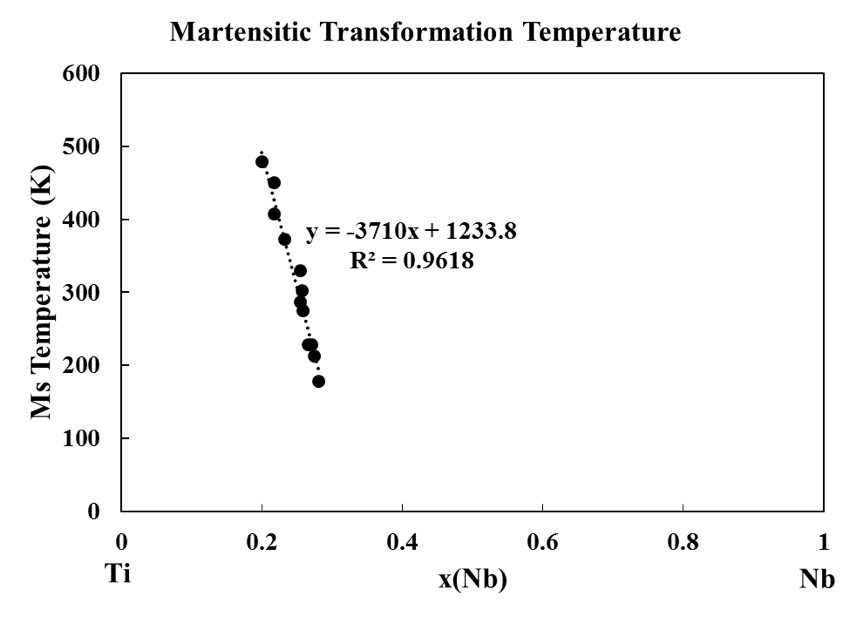
\includegraphics[width=\textwidth]{Chapter-7/Figures/tinbms.png}
	\caption{Martensitic transformation temperature is plotted versus the Ti-Nb composition.}
	\label{Ch7-figure:titnbms}
\end{figure}

\pagebreak
\begin{figure}[H]
	\centering
	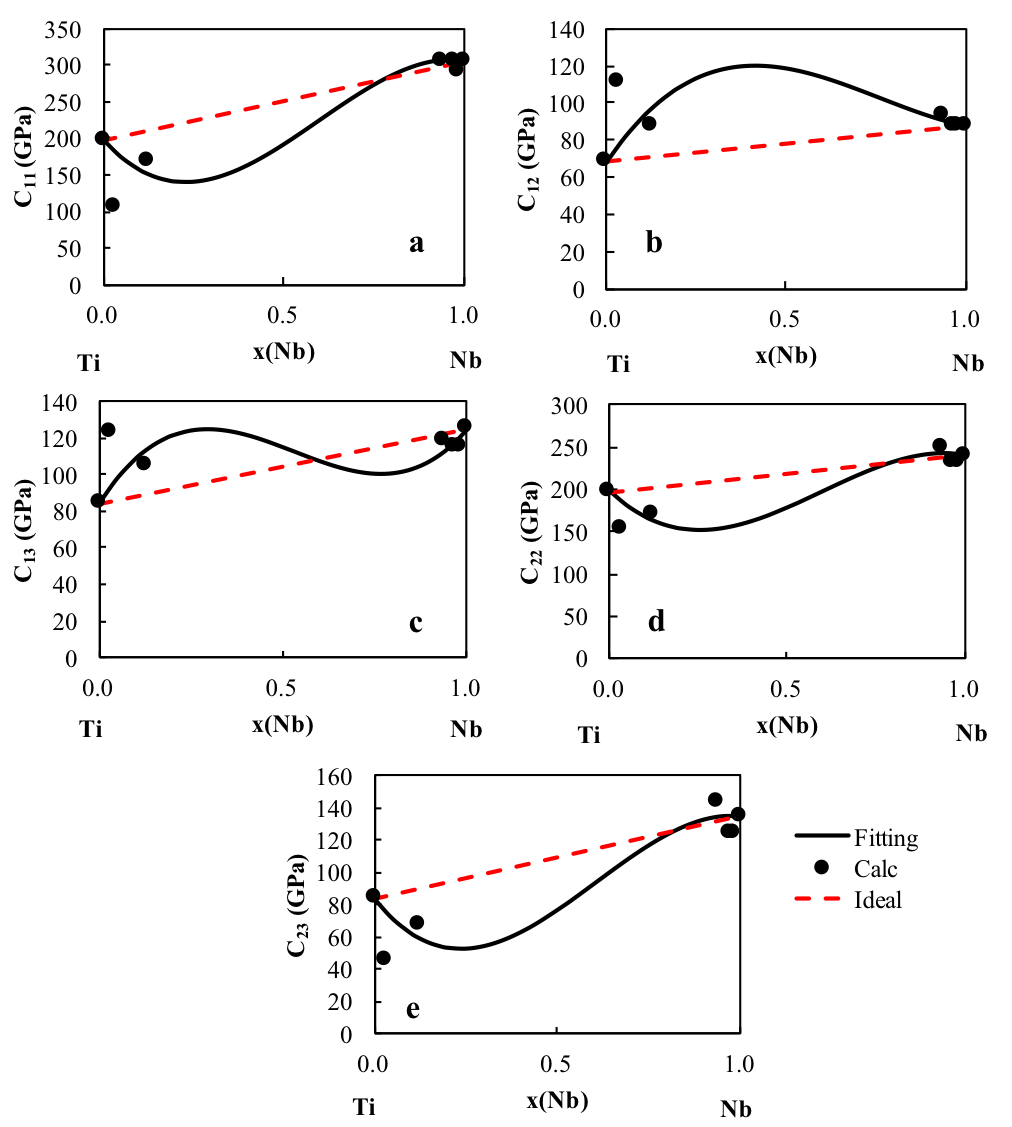
\includegraphics[width=\textwidth]{Chapter-7/Figures/adpe1.png}
	\caption{Calculated $c_{11}$, $c_{12}$, $c_{13}$, $c_{22}$, and  $c_{23}$ values (circles) plotted with the linear combination of the pure elements (red dashed line) and the present modeling (black solid line) for five of the elastic stiffness constants of Ti-Nb in the $\alpha"$ phase.}
	\label{Ch7-figure:adpelas1}
\end{figure}

\pagebreak
\begin{figure}[H]
	\centering
	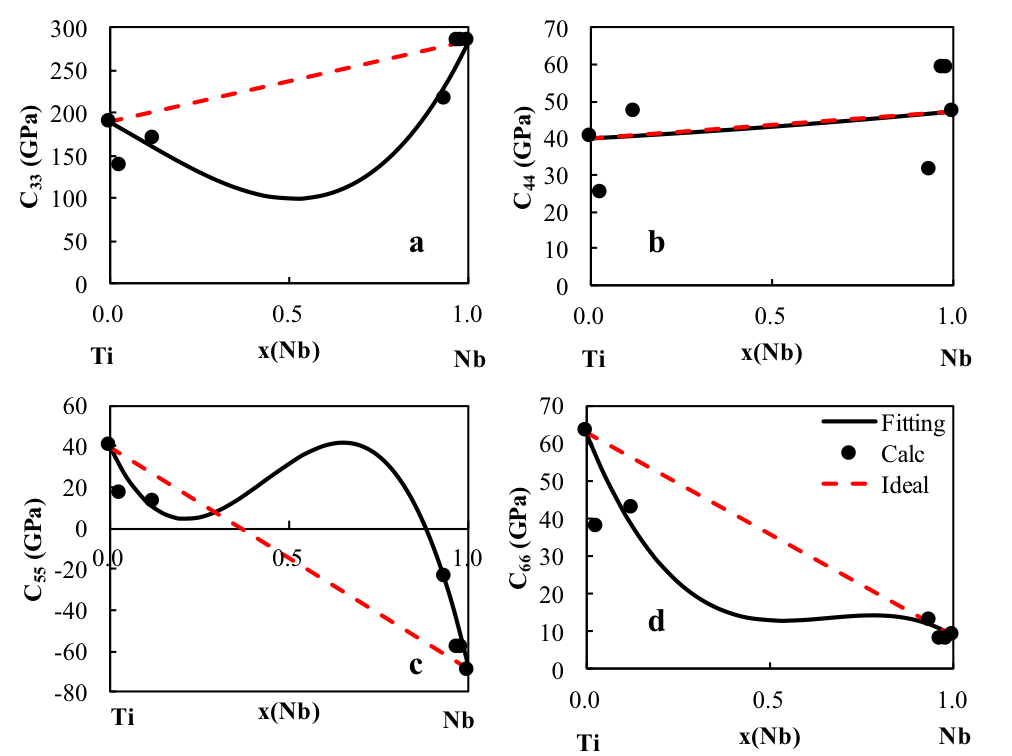
\includegraphics[width=\textwidth]{Chapter-7/Figures/adpe2.png}
	\caption{Calculated $c_{33}$, $c_{44}$, $c_{55}$, and $c_{66}$ values (circles) plotted with the linear combination of the pure elements (red dashed line) and the present modeling (black solid line) for four of the elastic stiffness constants of Ti-Nb in the $\alpha"$ phase.}
	\label{Ch7-figure:adpelas2}
\end{figure}

\pagebreak
\begin{figure}[H]
	\centering
	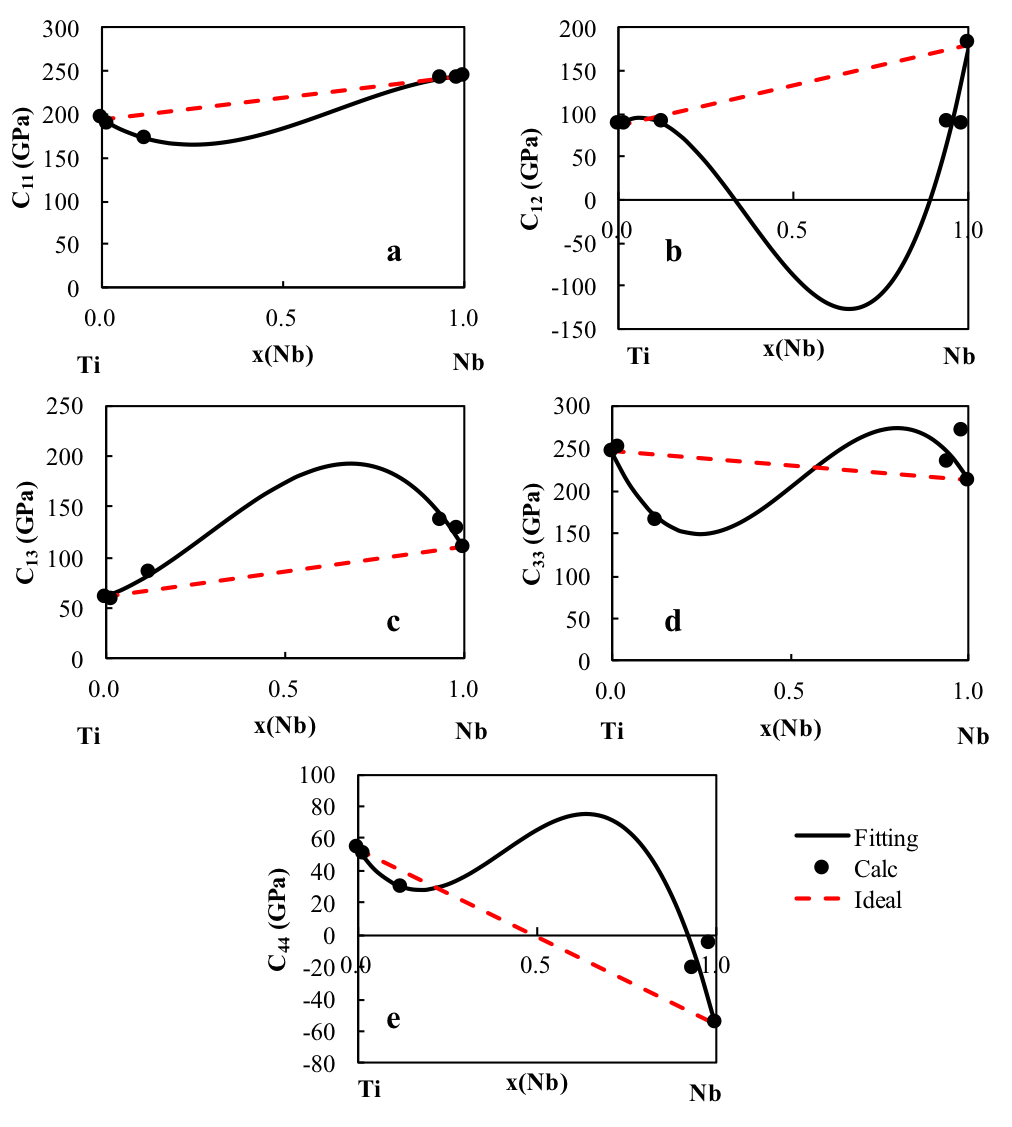
\includegraphics[width=\textwidth]{Chapter-7/Figures/omegae1.png}
	\caption{Calculated $c_{11}$, $c_{12}$, $c_{13}$, $c_{33}$, and $c_{44}$ values (circles) plotted with the linear combination of the pure elements (red dashed line) and the present modeling (black solid line) for the elastic stiffness constants of Ti-Nb in the $\omega$ phase.}
	\label{Ch7-figure:omegae1}
\end{figure}

\pagebreak
\begin{figure}[H]
	\centering
	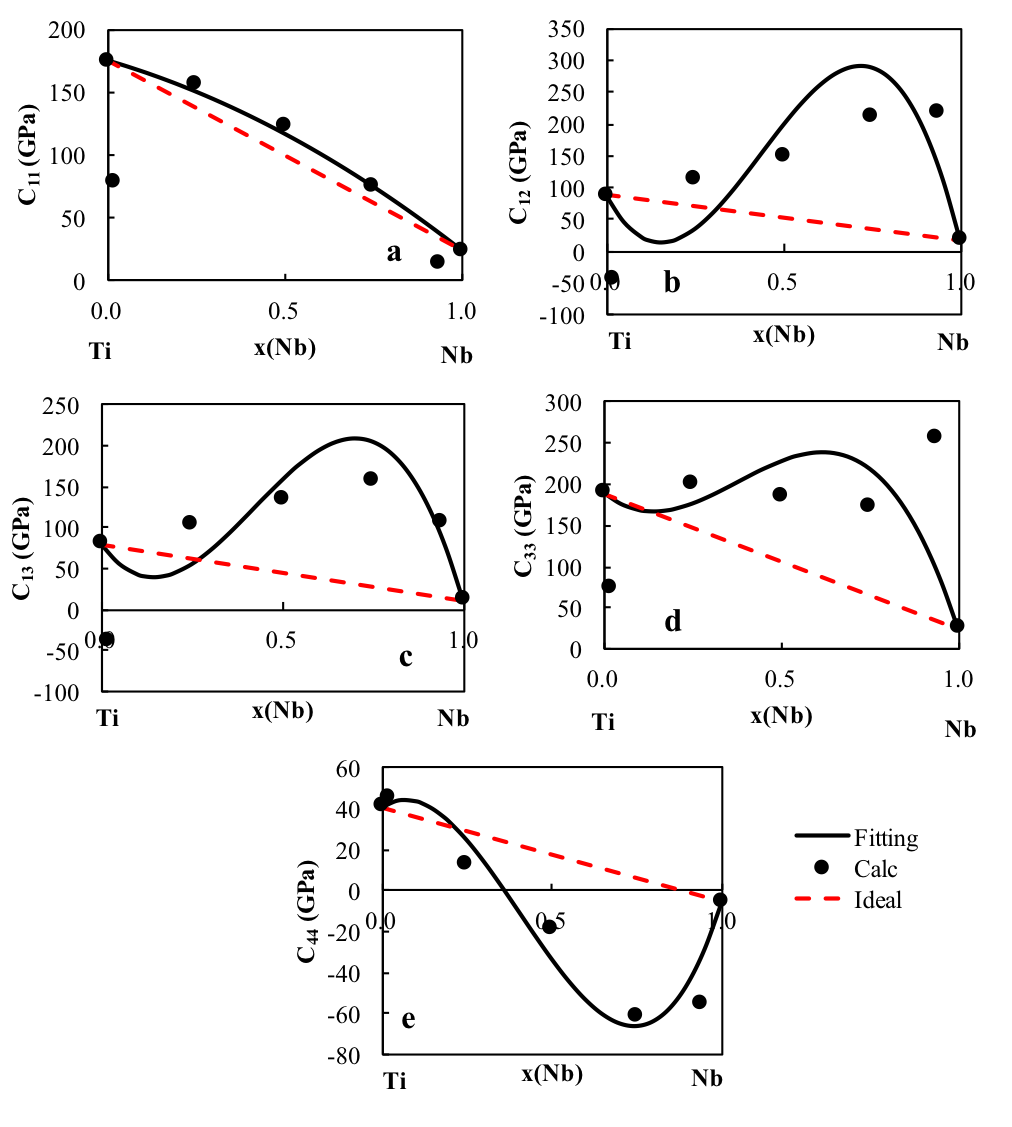
\includegraphics[width=\textwidth]{Chapter-7/Figures/hcpe1.png}
	\caption{Calculated $c_{11}$, $c_{12}$, $c_{13}$, $c_{33}$, and $c_{44}$ values (circles) plotted with the linear combination of the pure elements (red dashed line) and the present modeling (black solid line) for the elastic stiffness constants of Ti-Nb in the hcp phase.}
	\label{Ch7-figure:hcpe1}
\end{figure}

\pagebreak
\begin{figure}[H]
	\centering
	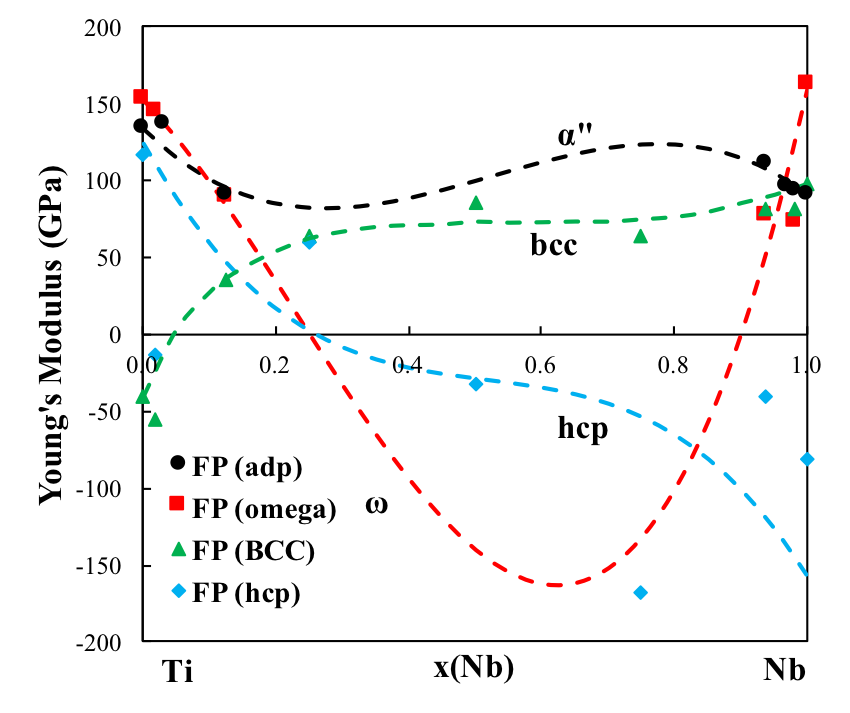
\includegraphics[width=\textwidth]{Chapter-7/Figures/tinbelastic.png}
	\caption{Elastic properites of the bcc, hcp, $\omega$, $\alpha"$ phases in the Ti-Nb system calculated from first-principles based on DFT are plotted as symbols. The CALPHAD fittings are plotted as the dashed lines. The figure is plotted from pure Ti to pure Nb.}
	\label{Ch7-figure:tinbelastic}
\end{figure}

\pagebreak
\begin{figure}[H]
	\centering
	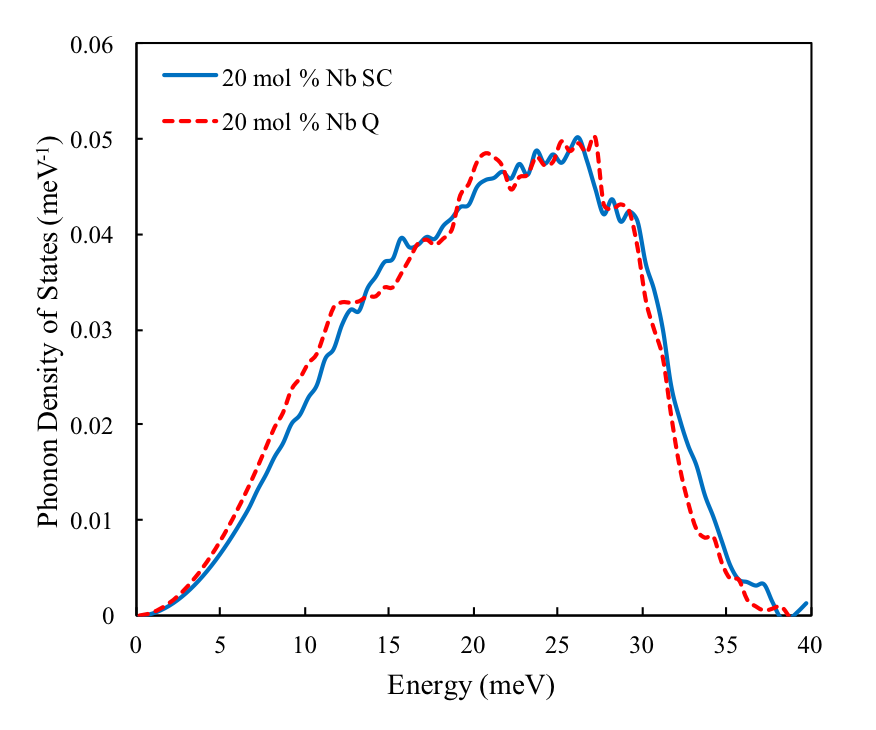
\includegraphics[width=\textwidth]{Chapter-7/Figures/50dos20.png}
	\caption{Phonon density of states for the Ti-Nb alloy at 20 at. \% Nb. The dashed line represents the slow cooled sample while the solid line represents the quenched sample.}
	\label{Ch7-figure:50dos20}
\end{figure}

\pagebreak
\begin{figure}[H]
	\centering
	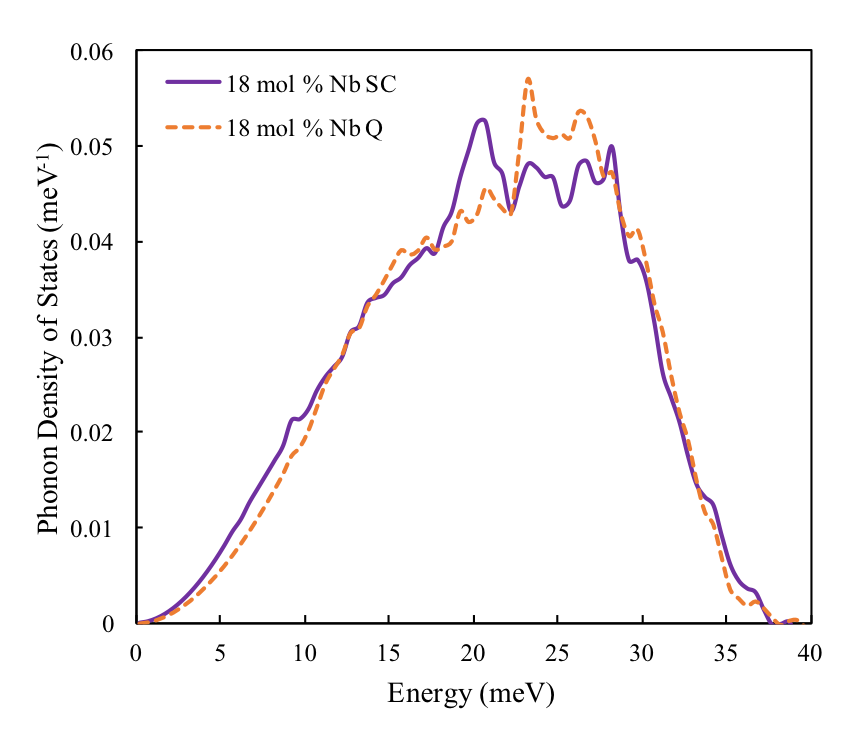
\includegraphics[width=\textwidth]{Chapter-7/Figures/50dos18.png}
	\caption{Phonon density of states for the Ti-Nb alloy at 18 at. \% Nb. The dashed line represents the slow cooled sample while the solid line represents the quenched sample.}
	\label{Ch7-figure:50dos18}
\end{figure}

\pagebreak
\begin{figure}[H]
	\centering
	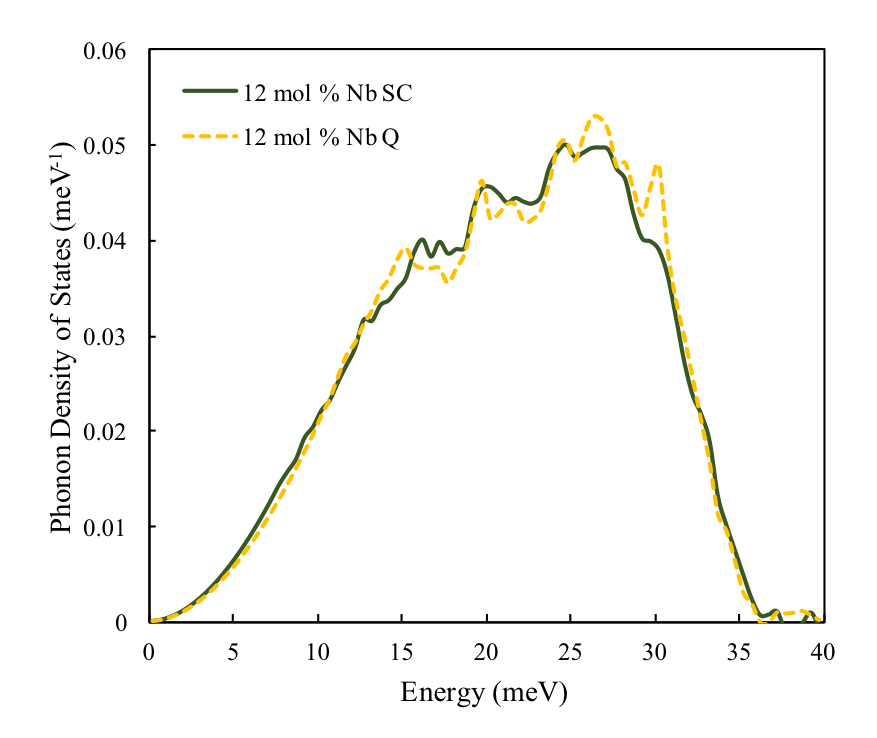
\includegraphics[width=\textwidth]{Chapter-7/Figures/50dos12.png}
	\caption{Phonon density of states for the Ti-Nb alloy at 12 at. \% Nb. The dashed line represents the slow cooled sample while the solid line represents the quenched sample.}
	\label{Ch7-figure:50dos12}
\end{figure}

\pagebreak
\begin{figure}[H]
	\centering
	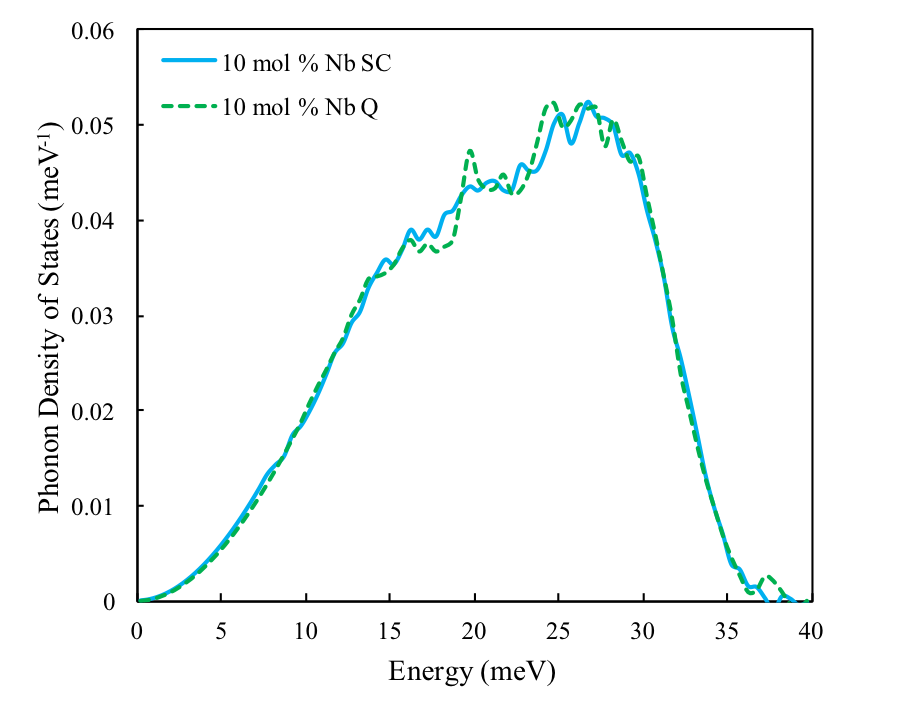
\includegraphics[width=\textwidth]{Chapter-7/Figures/50dos10.png}
	\caption{Phonon density of states for the Ti-Nb alloy at 10 at. \% Nb. The dashed line represents the slow cooled sample while the solid line represents the quenched sample.}
	\label{Ch7-figure:50dos10}
\end{figure}

\pagebreak
\begin{figure}[H]
	\centering
	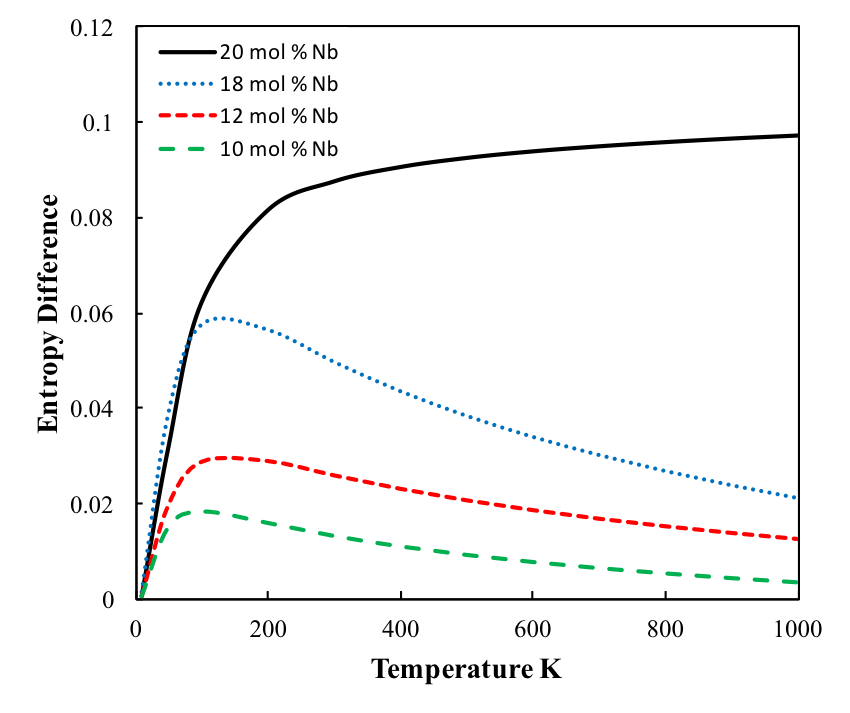
\includegraphics[width=\textwidth]{Chapter-7/Figures/ediff.png}
	\caption{Entropy difference between the Ti-Nb alloys with the same alloy composition as a function of temperature.}
	\label{Ch7-figure:ediff}
\end{figure}

\pagebreak
\begin{figure}[H]
	\centering
	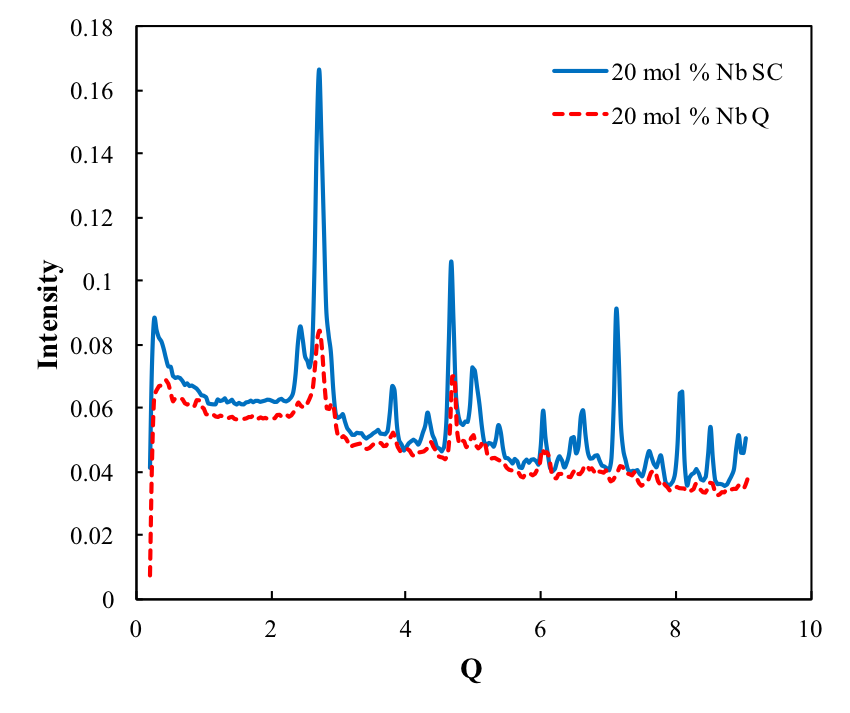
\includegraphics[width=\textwidth]{Chapter-7/Figures/50diff20.png}
	\caption{Diffraction pattern of the Ti-Nb alloy at 20 at. \% Nb. The dashed line represents the slow cooled sample while the solid line represents the quenched sample.}
	\label{Ch7-figure:50diff20}
\end{figure}

\pagebreak
\begin{figure}[H]
	\centering
	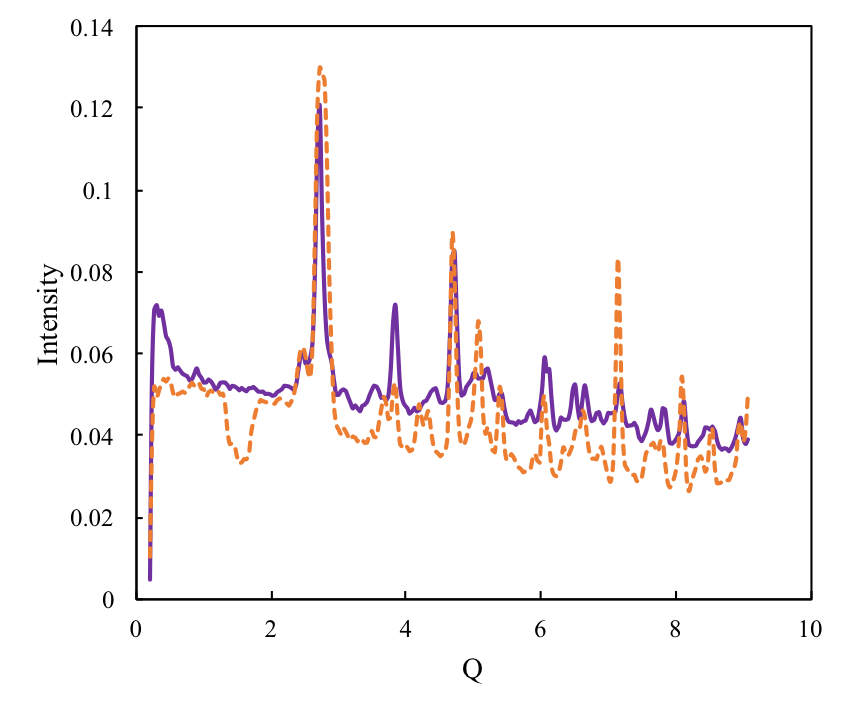
\includegraphics[width=\textwidth]{Chapter-7/Figures/50diff18.png}
	\caption{Diffraction pattern of the Ti-Nb alloy at 18 at. \% Nb. The dashed line represents the slow cooled sample while the solid line represents the quenched sample.}
	\label{Ch7-figure:50diff18}
\end{figure}

\pagebreak
\begin{figure}[H]
	\centering
	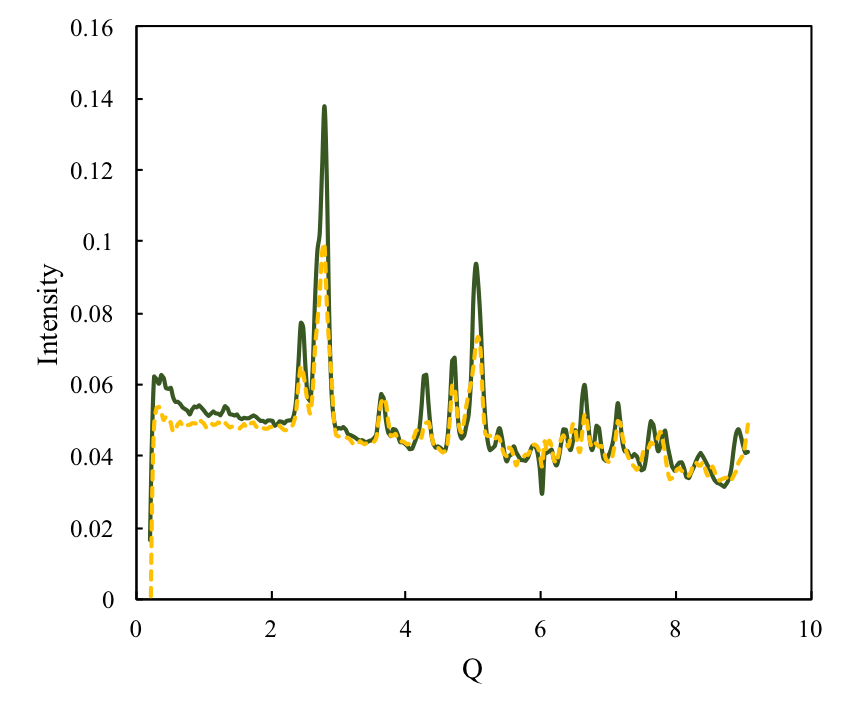
\includegraphics[width=\textwidth]{Chapter-7/Figures/50diff12.png}
	\caption{Diffraction pattern of the Ti-Nb alloy at 12 at. \% Nb. The dashed line represents the slow cooled sample while the solid line represents the quenched sample.}
	\label{Ch7-figure:50diff12}
\end{figure}

\pagebreak
\begin{figure}[H]
	\centering
	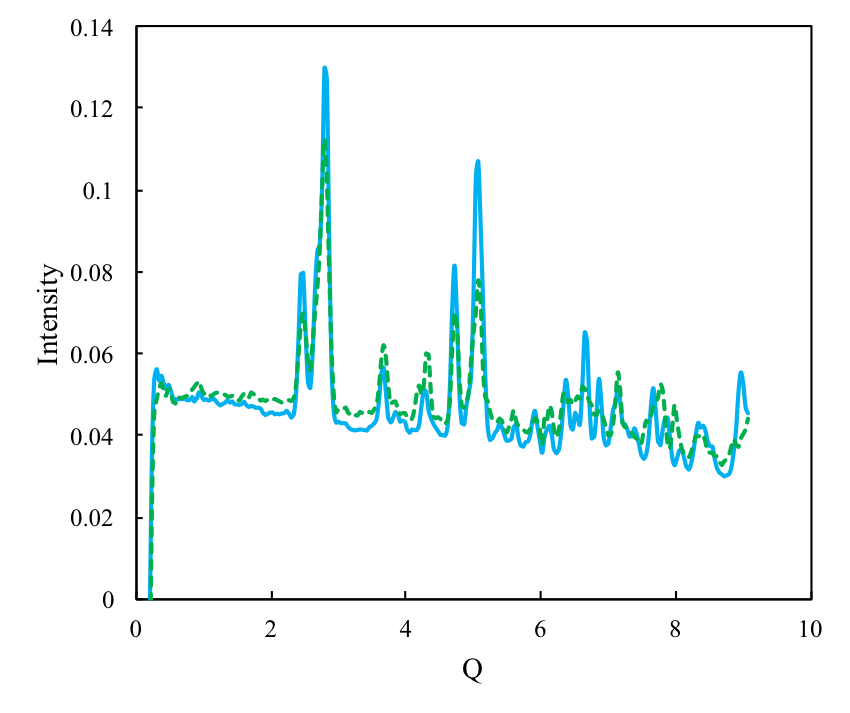
\includegraphics[width=\textwidth]{Chapter-7/Figures/50diff10.png}
	\caption{Diffraction pattern of the Ti-Nb alloy at 10 at. \% Nb. The dashed line represents the slow cooled sample while the solid line represents the quenched sample.}
	\label{Ch7-figure:50diff10}
\end{figure}